% !TEX TS-program = xelatex
% !TEX encoding = UTF-8 Unicode

\documentclass[AutoFakeBold]{LZUThesis}
\usepackage{wasysym}
\usepackage{enumitem}
\usepackage[most]{tcolorbox}
\usepackage{multirow}
\usepackage{tikz}
\usetikzlibrary{arrows.meta, decorations.markings}
\usepackage{hyperref}
\usepackage[numbers,sort&compress]{natbib}
\newcommand{\upcite}[1]{\textsuperscript{\textsuperscript{\cite{#1}}}}
\allowdisplaybreaks[4]

% for verilog code coloring
\definecolor{vgreen}{RGB}{104,180,104}
\definecolor{vblue}{RGB}{49,49,255}
\definecolor{vorange}{RGB}{255,143,102}

\lstdefinestyle{verilog-style}
{
    language=Verilog,
    basicstyle=\small\ttfamily,
    keywordstyle=\color{vblue},
    identifierstyle=\color{black},
    commentstyle=\color{vgreen},
    numbers=left,
    numberstyle=\tiny\color{black},
    numbersep=10pt,
    tabsize=8,
    moredelim=*[s][\colorIndex]{[}{]},
    literate=*{:}{:}1
}

\makeatletter
\newcommand*\@lbracket{[}
\newcommand*\@rbracket{]}
\newcommand*\@colon{:}
\newcommand*\colorIndex{%
    \edef\@temp{\the\lst@token}%
    \ifx\@temp\@lbracket \color{black}%
    \else\ifx\@temp\@rbracket \color{black}%
    \else\ifx\@temp\@colon \color{black}%
    \else \color{vorange}%
    \fi\fi\fi
}
\makeatother

\usepackage{trace}

\begin{document}

\title{{实验三 寄存器堆的实现}}

\entitle{Experiment 3 Implementation of Register File}

\author{生物信息学班 李泽华 320210928501}
\major{计算机组成原理}
\advisor{高平}
\college{生命科学学院}
\grade{2021级}


\frontmatter

% \ZhAbstract{
% }{
% }

%\EnAbstract{
%}{
%}

%\customcontent

\mainmatter

% \chapter{\texorpdfstring{绪 \quad 论}{绪论}}
\chapter{实验目的}
\begin{enumerate}
    \item 熟悉并掌握 MIPS 计算机中寄存器堆的原理和设计方法。
    \item 初步了解 MIPS 指令结构和源操作数/目的操作数的概念。
    \item 熟悉并运用 verilog 语言进行电路设计。
    \item 为后续设计 cpu 的实验打下基础
\end{enumerate}

\chapter{实验任务与要求}
\section{实验任务}
\begin{enumerate}
    \item 学习 MIPS 计算机中寄存器堆的设计及原理,如:有多少个寄存器,有无特殊设置的寄存器,mips 指令如何去索引寄存器的等。
    \item 自行设计本次实验的方案,画出结构框图,详细标出输入输出端口,本次实验建议设计为异步读同步写的寄存器堆,即读寄存器不需要时钟控制,但写寄存器需时钟控制。
    \item 本次实验建议寄存器堆设计为 1 个写端口和 2 个读端口,后续 CPU 实验用到的寄存器堆需要 1 个写端口和 2 个读端口。
    \item 根据设计的实验方案,使用 verilog 编写相应代码。
    \item 对编写的代码进行仿真,得到正确的波形图。
    \item 将以上设计作为一个单独的模块,设计一个外围模块去调用该模块。外围模块中需调用封装好的 LCD 触摸屏模块,显示寄存器堆的读写端口地址和数据,最好能扫描出所有寄存器的值显示在 LCD 触摸屏上,并且需要利用触摸功能输入寄存器堆的读写地址和写数据。
    \item 将编写的代码进行综合布局布线,并下载到实验箱中的 FPGA 板子上进行演示。
\end{enumerate}
\section{实验要求}
\begin{enumerate}
    \item 做好预习:
    1) 掌握寄存器堆的工作原理;
    2) 确定寄存器堆的输入输出端口设计;
    3) 在课前画好寄存器堆的设计框图或实验原理图;
    \item 实验实施:
    1) 确认寄存器堆的设计框图的正确性;
    2) 编写 verilog 代码;
    3) 对该模块进行仿真,得出正确的波形,截图作为实验报告结果一项的材料;
    4) 完成调用寄存器堆模块的外围模块的设计,并编写代码;
    5) 对代码进行综合布局布线下载到实验箱里 FPGA 板上,进行上板验证。
    \item 实验检查:
    1) 完成上板验证后,让指导老师或助教进行检查,进行现场演示,按照检查人员的要求,对特定寄存器读写,可对演示结果进行拍照作为实验报告结果一项的材料。
    \item 实验报告的撰写:
    1) 实验结束后,需按照规定的格式完成实验报告的撰写。
\end{enumerate}

\chapter{实验结果}
\section{R-S触发器}
\begin{figure}[htbp]
    \centering
    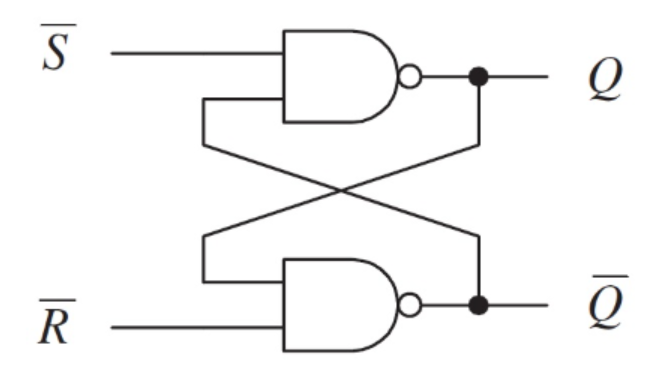
\includegraphics[width=0.4\textwidth]{img/RS_latch}
    \caption{R-S触发器}
\end{figure}

\begin{lstlisting}[style={verilog-style}]
/**
 * @brief R-S触发器
 * @param S 设置端set
 * @param R 重置端reset
 * @param Q 输出端
 * @param Q_bar 输出端的反相
 * 状态表:
    * R	S  | Q_n	Q_bar_n	    描述
    * 0	1  | 1	    Q_bar_n-1	设置Q为1
    * 1	0  | Q_n-1	1	        设置Q_bar为1
    * 1	1  | Q_n-1	Q_bar_n-1	保持前状态
    * 0	0  | 1	    1	        非法状态(禁止)
 */
module rs_nand_latch(R, S, Q);
    input R, S;
    output Q;

    wire Q_bar;

    nand n1(Q, S, Q_bar);
    nand n2(Q_bar, R, Q);

endmodule // r-s_nand_latch
\end{lstlisting}

\begin{figure}[htbp]
    \centering
    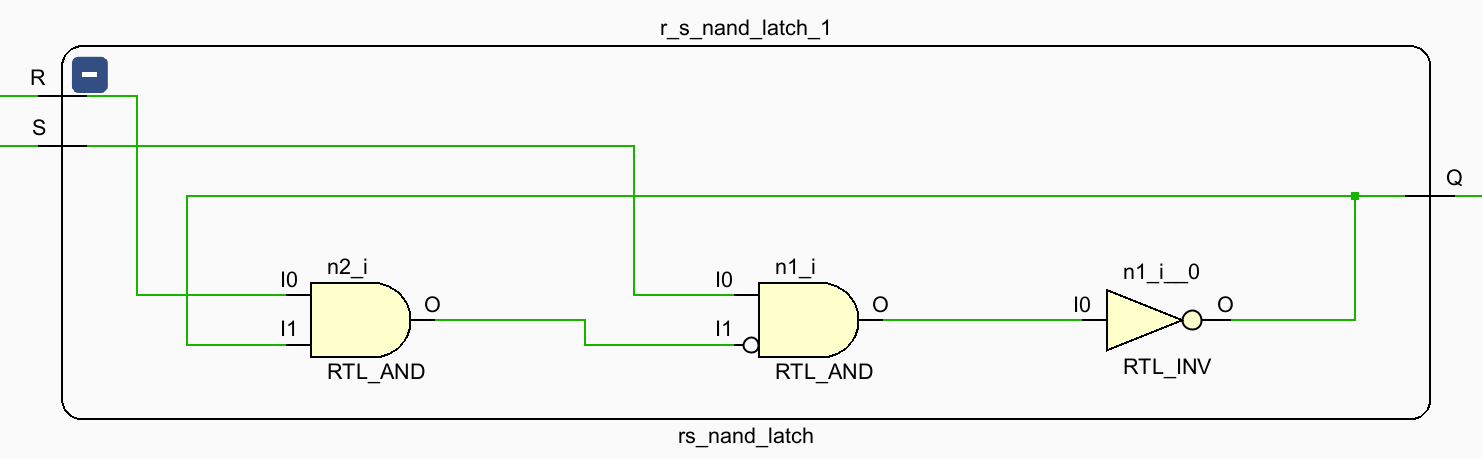
\includegraphics[width=0.4\textwidth]{img/RS_latch_ele}
    \caption{rs触发器 elaberate design}
\end{figure}

\section{D触发器}
\begin{figure}[htbp]
    \centering
    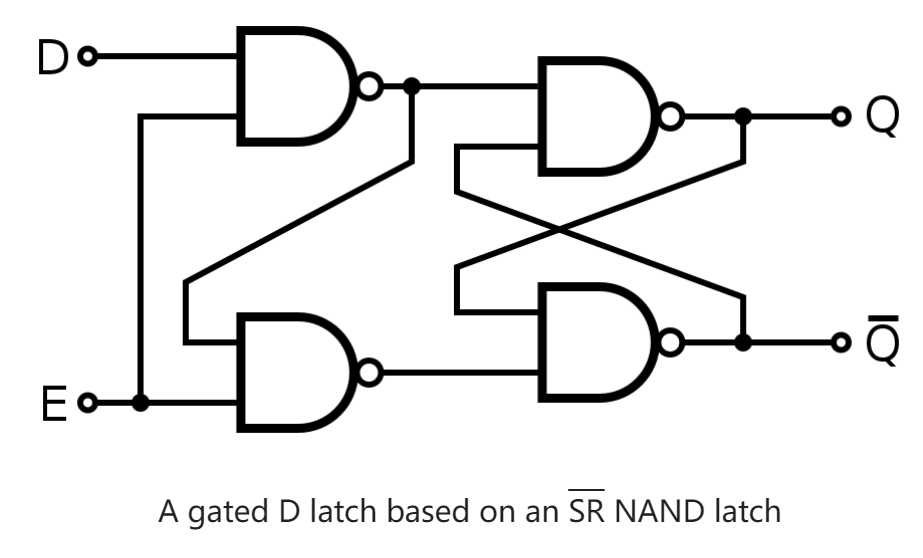
\includegraphics[width=0.4\textwidth]{img/D_latch}
    \caption{D触发器}
\end{figure}

\begin{lstlisting}[style={verilog-style}]
/**
 * @brief D触发器
 * @param D 数据端 data
 * @param E 使能端 enable
 * @param Q 输出端
 * @param Q_bar 输出端的反相
    * 状态表:
        * E	D  | Q_n	Q_bar_n	    描述
        * 0	X  | Q_n-1	Q_bar_n-1	保持前状态
        * 1	0  | 0	    1	        重置Q
        * 1	1  | 1	    0	        设置Q
 */
module d_latch(D, E, Q);
    input D, E;
    output Q;

    wire wire_1, wire_2;

    nand n1(wire_1, D, E);
    nand n2(wire_2, E, wire_1);

    rs_nand_latch r_s_nand_latch_1(wire_2, wire_1, Q);
endmodule // d_latch
\end{lstlisting}

\section{D触发器}
\begin{figure}[htbp]
    \centering
    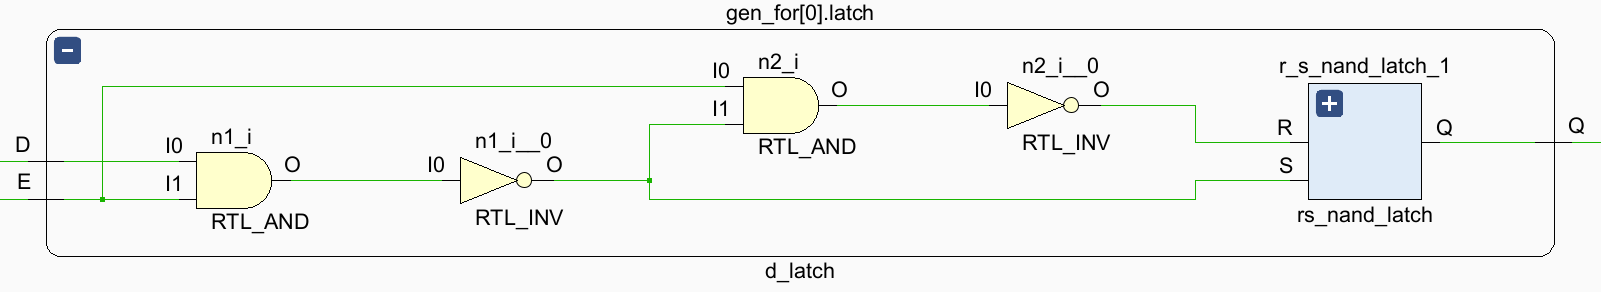
\includegraphics[width=0.4\textwidth]{img/D_latch_ele}
    \caption{D触发器 elaberate design}
\end{figure}

\section{寄存器}
\begin{lstlisting}[style={verilog-style}]
/**
 * @brief 32位寄存器
 */
module register_32bit(D, E, Q);
    input [31:0] D;    // 32-bit data input
    input E;          // Enable signal (common for all latches)
    output [31:0] Q;   // 32-bit data output

    // Instantiate 32 D latches, one for each bit
    // d_latch latches[31:0] (
    //     .D(D), 
    //     .E(E), 
    //     .Q(Q)
    // );
    genvar i;
    generate
        for (i = 0; i < 32; i = i + 1) begin: gen_for
            d_latch latch(
                .D(D[i]), 
                .E(E), 
                .Q(Q[i])
            );
        end
    endgenerate

endmodule // register_32bit
\end{lstlisting}

\begin{figure}[htbp]
    \centering
    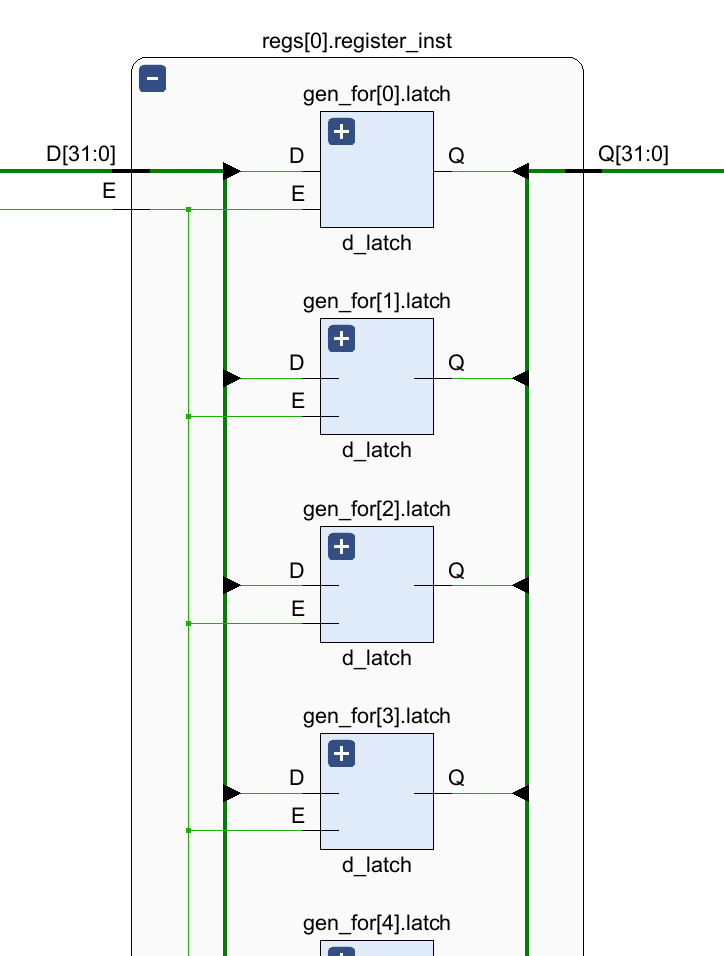
\includegraphics[width=0.4\textwidth]{img/register_ele}
    \caption{32位寄存器 elaberated design}
\end{figure}

\section{32位寄存器}

\section{寄存器堆}
\begin{lstlisting}[style={verilog-style}]
module regfile(clk, rst, we, waddr, wdata, raddr1, rdata1, raddr2, rdata2, test_addr, test_data);
    input clk;                  // 时钟信号 clock
    input rst;                  // 复位信号 reset
    input we;                   // 写使能信号 write enable
    input [4:0] waddr;          // 写地址 write address
    input [31:0] wdata;         // 写数据 write data
    input [4:0] raddr1;         // 读地址1 read address 1
    input [4:0] raddr2;         // 读地址2 read address 2
    input [4:0] test_addr;      // 测试地址 test address
    output [31:0] rdata1;       // 读数据1 read data 1
    output [31:0] rdata2;       // 读数据2 read data 2
    output [31:0] test_data;    // 测试数据 test data
    

    reg enable[31:0];
    wire [31:0] reg_outputs[31:0];

    integer i;
    always @(posedge clk) begin  // 时钟上升沿触发
        // 复位时,将所有寄存器的使能信号置0
        if (rst) begin
            for (i = 0; i < 32; i = i + 1) begin
                enable[i] <= 0; // 非阻塞赋值
            end
        end else begin
            // we为1且地址等于waddr时,使能信号为1
            for (i = 0; i < 32; i = i + 1) begin
                if (we && i == waddr) begin
                    enable[i] <= 1;
                end else begin
                    enable[i] <= 0;
                end
            end
        end
    end

    // 32个32位寄存器
    genvar j;
    generate
        for (j = 0; j < 32; j = j + 1) begin : regs
            register_32bit register_inst (
                .D(wdata),
                .E(enable[j]),
                .Q(reg_outputs[j])
            );
        end
    endgenerate

    // 读数据
    assign rdata1 = reg_outputs[raddr1];
    assign rdata2 = reg_outputs[raddr2];

    // 测试数据, 读出寄存器的值显示在触摸屏上
    assign test_data = reg_outputs[test_addr];

endmodule //regfile

\end{lstlisting}

\section{tb}
\begin{lstlisting}[style={verilog-style}]
module tb_regfile;

    // Inputs
    reg clk;
    reg rst;
    reg we;
    reg [4:0] waddr;
    reg [31:0] wdata;
    reg [4:0] raddr1;
    reg [4:0] raddr2;

    // Outputs
    wire [31:0] rdata1;
    wire [31:0] rdata2;

    // Instantiate the regfile module
    regfile uut (
        .clk(clk),
        .rst(rst),
        .we(we),
        .waddr(waddr),
        .wdata(wdata),
        .raddr1(raddr1),
        .rdata1(rdata1),
        .raddr2(raddr2),
        .rdata2(rdata2)
    );

    // 生成时钟信号
    initial begin
        clk = 0;
        forever #5 clk = !clk;  // Generate a clock with 10 ns period
    end

    // Test cases
    initial begin
        // Initialize Inputs
        rst = 1; we = 0; waddr = 0; wdata = 0; raddr1 = 0; raddr2 = 0;

        // Apply reset
        #20 rst = 0;  // 释放复位信号,确保至少两个时钟周期内的状态

        // Wait for reset to propagate
        #10;

        // Case 1: 读写同一地址
        we = 1; waddr = 5; wdata = 32'hAAAA_BBBB;
        #10;  // Wait a clock cycle for write to complete
        we = 0; raddr1 = 5; raddr2 = 5;
        #10;  // Wait a clock cycle to read the data

        // Case 2: 读写不同地址
        #10; we = 1; waddr = 15; wdata = 32'h1234_5678;
        #10; we = 0; raddr1 = 15; raddr2 = 5;  // Read new data and previous data

        // Case 3: 不写入数据是否保持不变
        #20; raddr1 = 15; raddr2 = 5;

        #10 $finish;
    end

endmodule // tb_regfile
    
\end{lstlisting}

\section{仿真结果}

\begin{figure}[htbp]
    \centering
    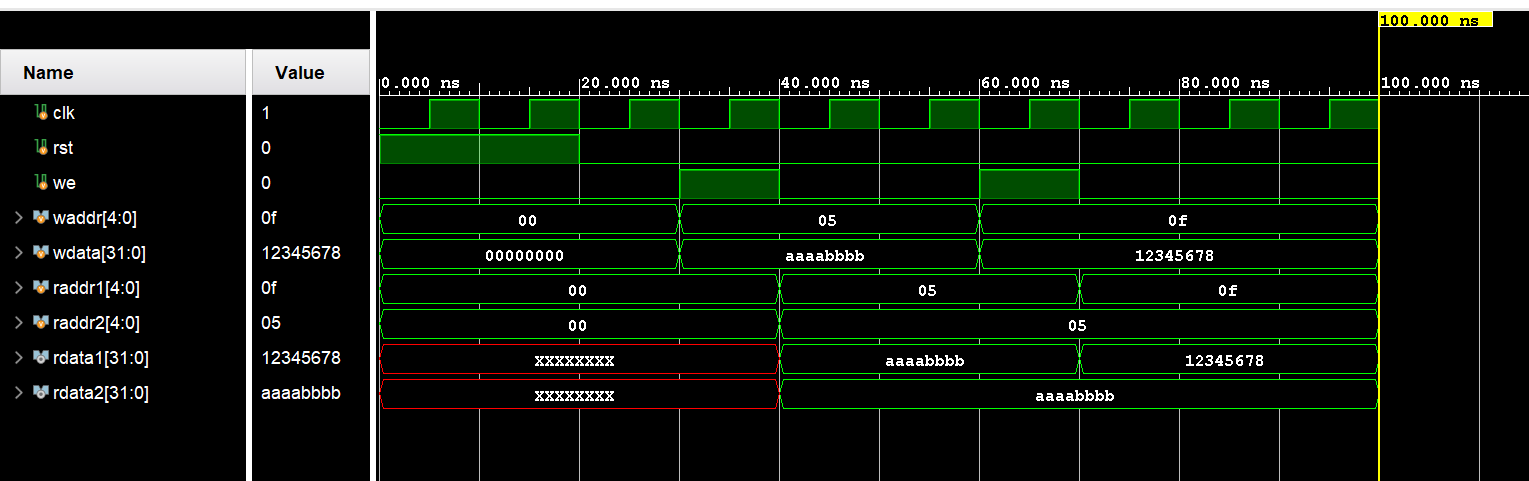
\includegraphics[width=0.8\textwidth]{img/sim_wave}
    \caption{仿真结果}
    \label{fig:sim}
\end{figure}
30ns - 40ns: 将write enable(we)置为1, 在waddr(05)寄存器写入wdata(aaaabbbb)

40ns - 60ns: 两个读数据口raddr1, raddr2同时置为05, rdata1, rdata2成功读取数据aaaabbbb

60ns - 70ns: 将we置为1, 在waddr(0f)寄存器中写入wdata(12345678)

70ns - 100ns: 两个独守巨口raddr1, raddr2一个置为0f, 一个置为05, rdata1, rdata2成功分别读取数据12345678和aaaabbbb

%\chapter{思考与讨论}
%\section{课后问题}
%论文后部
\backmatter


%=======%
%引入参考文献文件
%=======%
%\bibdatabase{bib/database}%bib文件名称 仅修改bib/ 后部分
%\printbib
%\nocite{*} %显示数据库中有的,但是正文没有引用的文献



\Appendix
参考链接:
\url{https://github.com/zehua0417/ComputerOrganizationAndArchitecture_exp}
\begin{figure}[htbp]
    \centering
    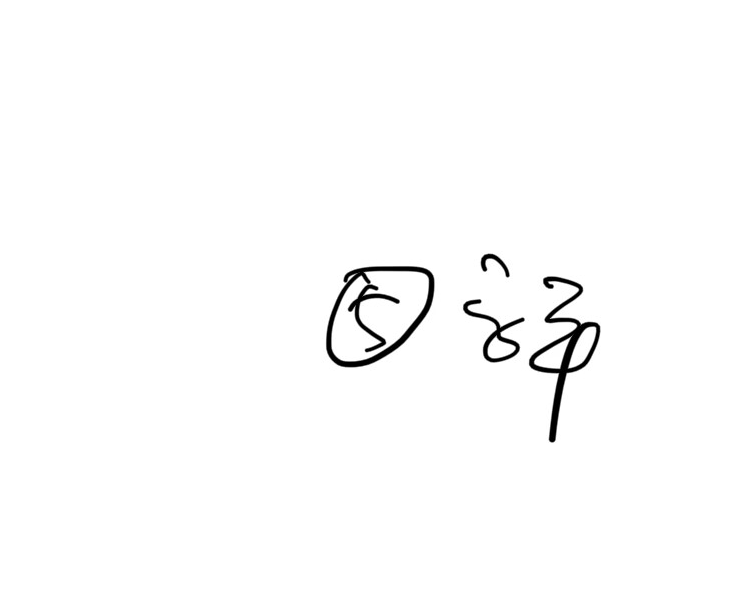
\includegraphics[width=0.4\textwidth]{img/sign}
\end{figure}

%\Thanks


%\Grade %这一句才是成绩页,上面是填写


\end{document}
